\documentclass[12pt,a4paper,onecolumn]{article}
\usepackage[utf8]{inputenc}
\usepackage[T1]{fontenc}
\usepackage[french]{babel}

% ------------------------- Color table ----------------------------------------
\usepackage{multirow}
\usepackage[table]{xcolor}
\definecolor{maroon}{cmyk}{0,0.87,0.68,0.32}
% ------------------------------------------------------------------------------

\usepackage{amscd}
\usepackage{amsthm}
\usepackage{physics}
\usepackage[left=2.2cm,right=2.2cm,top=2cm,bottom=2cm]{geometry}
\usepackage{textcomp,gensymb} %pour le °C, et textcomp pour éviter les warning
\usepackage{graphicx} %pour les images
\usepackage{caption}
\usepackage{subcaption}
\usepackage[colorlinks=true,
	breaklinks=true,
	citecolor=blue,
	linkcolor=blue,
	urlcolor=blue]{hyperref} % pour insérer des liens
\usepackage{epstopdf} %converting to PDF
\usepackage[export]{adjustbox} %for large figures

\usepackage{array}
\usepackage{dsfont}% indicatrice : \mathds{1}


% -------------------------- Mathematics ---------------------------------------
\graphicspath{{images/}} % For the images path
% ------------------------------------------------------------------------------

% -------------------------- Mathematics ---------------------------------------
\usepackage{mathrsfs, amsmath, amsfonts, amssymb}
\usepackage{bm}
\usepackage{mathtools}
\usepackage[Symbol]{upgreek} % For pi \uppi different from /pi
\newcommand{\R}{\mathbb{R}} % For Real space
% ------------------------------------------------------------------------------


% -------------------------- Code format ---------------------------------------
\usepackage[numbered,framed]{matlab-prettifier}
\lstset{
	style              = Matlab-editor,
	basicstyle         = \mlttfamily,
	escapechar         = '',
	mlshowsectionrules = true,
}
% ------------------------------------------------------------------------------

% ------------------------- Blbiographie --------------------------------------
% \usepackage[backend=biber, style=science]{biblatex}
% \addbibresource{biblio.bib}
% ------------------------------------------------------------------------------


\setcounter{tocdepth}{4} %Count paragraph
\setcounter{secnumdepth}{4} %Count paragraph
\usepackage{float}

\usepackage{graphicx} % for graphicspath
% \graphicspath{{../images/}}

\usepackage{array,tabularx}
\newcolumntype{L}[1]{>{\raggedright\let\newline\\\arraybackslash\hspace{0pt}}m{#1}}
\newcolumntype{C}[1]{>{\centering\let\newline\\\arraybackslash\hspace{0pt}}m{#1}}
\newcolumntype{R}[1]{>{\raggedleft\let\newline\\\arraybackslash\hspace{0pt}}m{#1}}

\newcommand{\assignmenttitle}{}
\newcommand{\studentname}{}
\newcommand{\email}{}
\newcommand{\schoolyear}{2017/2018}


\title{
\normalfont \normalsize 
\textsc{Object recognition and computer vision, Master MVA, \schoolyear} \\
[10pt] 
\rule{\linewidth}{0.5pt} \\[6pt] 
\huge \assignmenttitle \\
\rule{\linewidth}{2pt}  \\[10pt]
}

\author{\studentname}

\date{\small\email}

\newcommand{\question}[1]{\subsubsection*{#1}}

\setlist[enumerate]{topsep=0pt,itemsep=-1ex,partopsep=1ex,parsep=1ex,label=(\roman*)}

\graphicspath{{images/}}

\newcommand{\labelnotempty}[1]{
\def\temp{#1}\ifx\temp\empty
\else
    \label{#1}
\fi
}
% single figure
\newcommand{\singlefig}[4]{
\begin{figure}[ht!]
        \centering
        \includegraphics[width={#2}\columnwidth]{#1}
        \caption{#3}
        \labelnotempty{#4}
\end{figure}}

\newcommand{\subfig}[4]{
\includegraphics[width={#2}\columnwidth]{#1}
\caption{#3}
\labelnotempty{#4}
}

% double figure
\newcommand{\doublefig}[4]{
\begin{figure}[ht!]
    \centering
    \begin{subfigure}[t]{0.45\columnwidth}
        \centering
    #1
    \end{subfigure}
    ~
    \begin{subfigure}[t]{0.45\columnwidth}
        \centering
    #2
    \end{subfigure}
    \caption{#3}
    \labelnotempty{#4}
\end{figure}}

% triple figure
\newcommand{\triplefig}[5]{
\begin{figure}[ht!]
    \centering
    \begin{subfigure}[t]{0.30\columnwidth}
        \centering
    #1
    \end{subfigure}
    ~
    \begin{subfigure}[t]{0.30\columnwidth}
        \centering
    #2
    \end{subfigure}
    ~
    \begin{subfigure}[t]{0.30\columnwidth}
        \centering
    #3
    \end{subfigure}
    \caption{#4}
    \labelnotempty{#5}
\end{figure}}



% ------------------------ General informations --------------------------------
\title{Matrice Fondamentale}
\author{Vincent Matthys}
\graphicspath{{images/}}
% ------------------------------------------------------------------------------


\begin{document}

\begin{tabularx}{0.9\textwidth}{@{} l X r @{} }
	{\textsc{Master MVA}}               &  & \textsc{TP2}       \\
	\textsc{Sub-pixel image processing} &  & {ENS Paris Saclay} \\
\end{tabularx}
\vspace{1.5cm}
\begin{center}

	\rule[11pt]{5cm}{0.5pt}

	\textbf{\LARGE \textsc{Compte-rendu TP3}}
	\vspace{0.5cm}

	Vincent Matthys

	vincent.matthys@ens-paris-saclay.fr

	\rule{5cm}{0.5pt}

	\vspace{1.5cm}
\end{center}

\section{Exercice 6}

\begin{figure}[H]
	\centering
	\begin{subfigure}[b]{\textwidth}
		\centering
		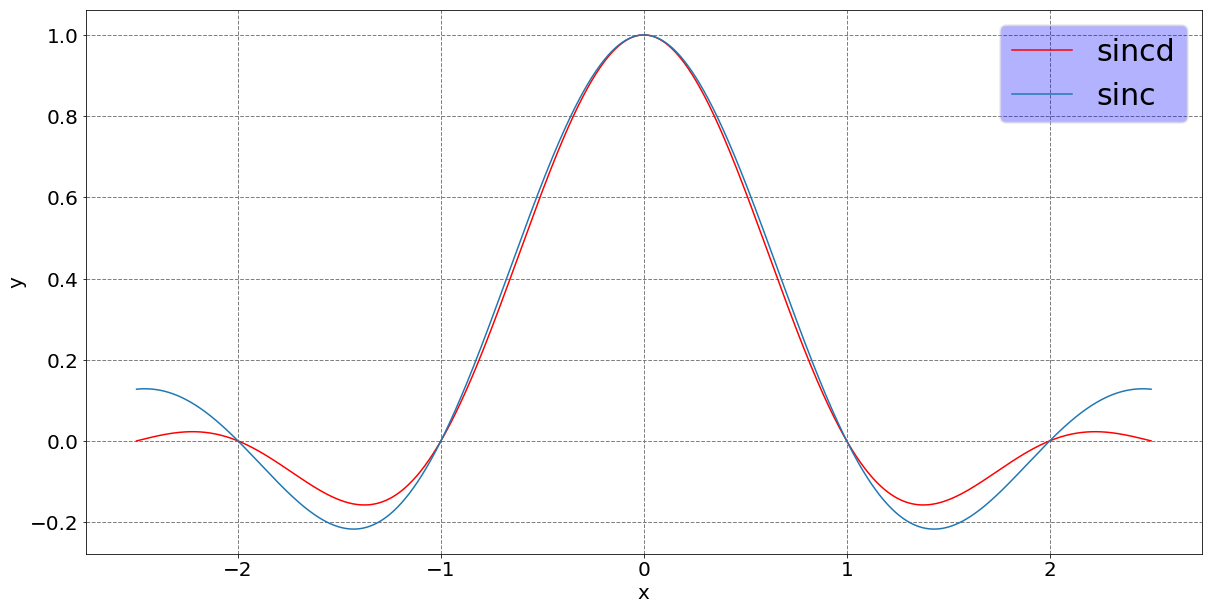
\includegraphics[height = 0.25\textheight]{6_5}
		\subcaption{Pour \(N = 5\)}
		\label{fig_6_5}
	\end{subfigure}
	\begin{subfigure}[b]{\textwidth}
		\centering
		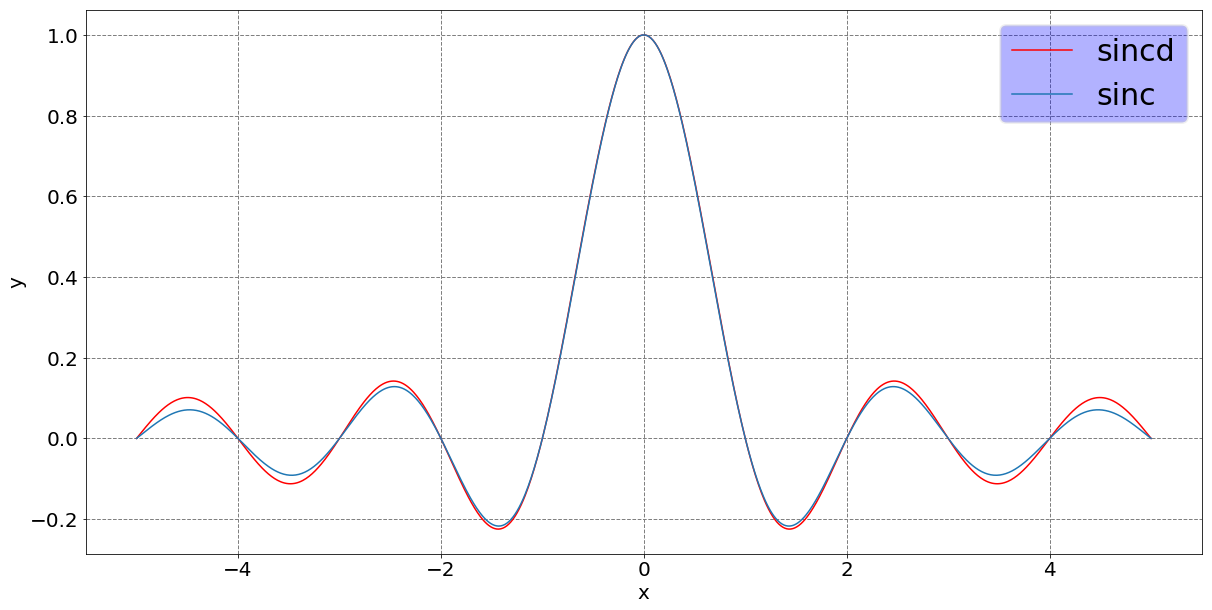
\includegraphics[height = 0.25\textheight]{6_10}
		\subcaption{Pour \(N = 10\)}
		\label{fig_6_10}
	\end{subfigure}
	\begin{subfigure}[b]{\textwidth}
		\centering
		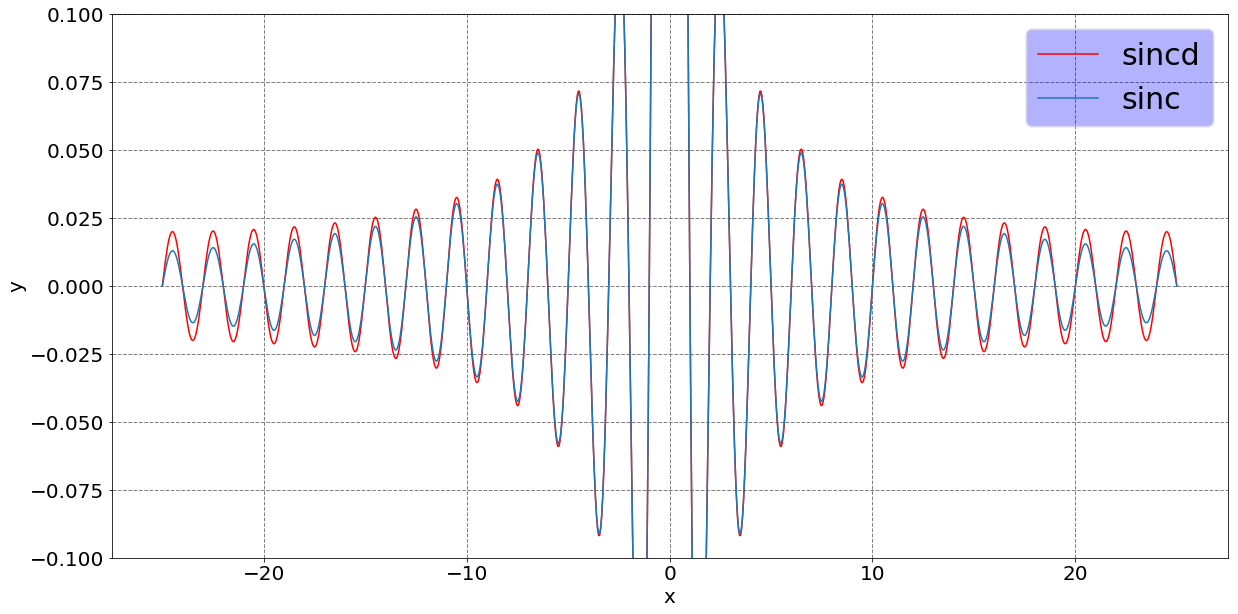
\includegraphics[height = 0.25\textheight]{6_50}
		\subcaption{Pour \(N = 50\)}
		\label{fig_6_50}
	\end{subfigure}
	\caption{Représentation graphique de la convergence du \(sincd_N\) et du \(sinc\), sur \([-N/2, N/2]\)}
	\label{fig_6}
\end{figure}

En figure~\ref{fig_6} sont représentés le \(sinc\) et le \(sincd_N\), pour différentes valeurs de \(N\) pour \(x \in[-N/2, N/2]\). On constate que, pour chaque valeur entière, on a bien égalité, et que, pour N assez grand, les différences sont minimes.

\section{Exercice 7}


\end{document}
